% This is samplepaper.tex, a sample chapter demonstrating the
% LLNCS macro package for Springer Computer Science proceedings;
% Version 2.20 of 2017/10/04
%
\RequirePackage{amsmath}
% \RequirePackage{amsthm}

\documentclass[runningheads]{llncs}


\usepackage[defaultlines=3,all]{nowidow}
%\usepackage{amsthm} %for customizing the theorem numbering
\usepackage{mathtools}
\usepackage{graphicx}
\usepackage{mathrsfs}
\usepackage{xcolor}
\usepackage{amssymb}
\usepackage{mathabx}
\usepackage{tikz}
\definecolor{cadmiumgreen}{rgb}{0.0, 0.42, 0.24}
\definecolor{dark-blue}{rgb}{0.05,0.25,1}
\usepackage[colorlinks=true,linkcolor={blue},citecolor=blue]{hyperref}
\usepackage[noabbrev,capitalise,nameinlink]{cleveref}
\usepackage[english]{babel}
\usepackage{microtype}
\usepackage{tcolorbox}

\usetikzlibrary{patterns,arrows,decorations.pathreplacing}


\newcommand{\Oof}{\mathcal{O}}
\newcommand{\Cc}{\mathscr{C}}
\newcommand{\Aa}{\mathcal{A}}
\newcommand{\Bb}{\mathcal{B}}
\newcommand{\Tt}{\mathcal{T}}
\newcommand{\Nn}{\mathcal{N}}
\newcommand{\Ss}{\mathcal{S}}
\newcommand{\Pp}{\mathcal{P}}
\newcommand{\Qq}{\mathcal{Q}}
\newcommand{\Rr}{\mathcal{R}}
\newcommand{\N}{\mathbb{N}}
\newcommand{\minor}{\preceq}
\newcommand{\red}[1]{\textcolor{red}{#1}}

% Used for displaying a sample figure. If possible, figure files should
% be included in EPS format.
%
% If you use the hyperref package, please uncomment the following line
% to display URLs in blue roman font according to Springer's eBook style:
% \renewcommand\UrlFont{\color{blue}\rmfamily}


% \theoremstyle{plain}
% 	\renewtheorem{theorem}{Theorem}[section]

% 	\newtheorem{lem}[theorem]{Lemma}
% 	\newtheorem{cor}[theorem]{Corollary}
% 	\newtheorem{cla}[theorem]{Claim}
% 	\newtheorem{prop}[theorem]{Proposition}
% 	\newtheorem*{exmp}{Example}
%   \newtheorem{rem}[theorem]{Remark}
%
% \theoremstyle{definition}
% 	\newtheorem{defn}[theorem]{Definition}
%

%\theoremstyle{remark}



% % % % % % % % % % % % % % % % % % % % % % % % % % % % % % % % % % % % % % % %
% % % % % % % % % % % % % % For commenting the text % % % % % % % % % % % % % %

% Add your name and pick a color !
%%% comments %%%
\newcommand{\commentmargin}[1]{\marginpar{\tiny\textit{#1}}}
\newcommand{\commenttext}[1]{ \begin{center} {\fbox{\begin{minipage}[h]{0.9 \linewidth}   {\textsf{ #1}} \end{minipage} }} \end{center}}

% \newcommand{\alexL}[1]{{\color{green}\commenttext{Alex L.: #1}}}
% \newcommand{\alexLmargin}[1]{{\commentmargin{\color{green}Alex L.: #1}}}

\newcommand{\alex}[1]{{\color{blue}\commenttext{Alex: #1}}}
\newcommand{\alexmargin}[1]{\commentmargin{\color{blue}Alex: #1}}


\newcommand{\sebi}[1]{{\color{red}\commenttext{Sebastian: #1}}}
\newcommand{\sebimargin}[1]{\commentmargin{\color{red}Sebastian: #1}}
% % % % % % % % % % % % % % % % % % % % % % % % % % % % % % % % % % % % % % % %
% % % % % % % % % % % % % % End Comments % % % % % % % % % % % % %



\begin{document}
%
\title{Constant round distributed domination on \newline graph classes with bounded expansion}
%
%\titlerunning{Abbreviated paper title}
% If the paper title is too long for the running head, you can set
% an abbreviated paper title here
%
\author{Simeon Kublenz\inst{1} \and
Sebastian Siebertz\inst{1}\orcidID{0000-0002-6347-1198} \and\\%\linebreak
Alexandre Vigny\inst{1}\orcidID{0000-0002-4298-8876}}
%
\authorrunning{S.\ Kublenz, S.\ Siebertz and A.\ Vigny}
% First names are abbreviated in the running head.
% If there are more than two authors, 'et al.' is used.
%
\institute{University of Bremen, Germany\\
\email{\{kublenz,siebertz,vigny\}@uni-bremen.de}}
%
\maketitle              % typeset the header of the contribution
%
% !TEX root = sirocco-main.tex

\begin{abstract}
We show that the dominating set problem admits a constant factor
approximation in a constant number of rounds in the \mbox{LOCAL} model
of distributed computing on graph classes with bounded \mbox{expansion}.
This generalizes a result of Czygrinow et al.\ for graphs with excluded
topological minors.

\keywords{Dominating set \and LOCAL algorithm \and Bounded expansion graph classes.}
\end{abstract}

% !TEX root = sirocco-main.tex

\section{Introduction}

A dominating set in an undirected and simple graph $G$ is a set
$D\subseteq V(G)$ such that every vertex $v\in V(G)$ either belongs
to $D$ or has a neighbor in $D$. The \textsc{Minimum Dominating Set} problem takes as input a graph $G$ and the objective
is to find a minimum size dominating set of~$G$. The decision
problem whether a graph admits a dominating set of size $k$
is NP-hard~\cite{karp1972reducibility} and this even holds in
very restricted settings, e.g. on planar graphs of maximum degree
$3$~\cite{garey1979computers}.

Consequently, attention
shifted from computing exact solutions to approxi\-mating
near optimal dominating sets. The simple greedy algorithm computes
an $\ln n$ approximation (where $n$ is number of vertices
of the input graph)
of a minimum dominating set \cite{johnson1974approximation,lovasz1975ratio}, and for
general graphs this algorithm is near optimal -- it is NP-hard
to approximate minimum dominating sets within factor
$(1-\epsilon)\ln n$ for every $\epsilon>0$~\cite{dinur2014analytical}.

Therefore, researchers tried to identify restricted
graph classes where better (sequential) approximations are possible. The problem
admits a PTAS on classes with sub\-exponential expansion~\cite{har2017approximation}. Here, expansion refers to the edge
density of bounded depth minors, which we will define in
detail below. Important examples of classes with subexponential
expansion include the class of planar graphs and more generally
classes that exclude some fixed graph as a minor. The dominating
set problem admits a constant factor approximation on classes of
bounded degeneracy (equivalently, of bounded arboricity)~\cite{bansal2017tight,lenzen2010minimum}
and an $\Oof(\ln \gamma)$ approxi\-mation (where~$\gamma$ denotes the size
of a minimum dominating set) on classes of bounded VC-dimension~\cite{bronnimann1995almost,even2005hitting}. In fact, the greedy
algorithm can be modified to yield a constant factor approximation on
graphs with bounded degeneracy~\cite{jones2017parameterized} and an $\Oof(\ln \gamma)$
approximation on biclique-free graphs (graphs that exclude some fixed
complete bipartite graph $K_{t,t}$ as a subgraph)~\cite{siebertz2019greedy}. However, it is unlikely
that polynomial-time constant factor approximations exist even on
$K_{3,3}$-free graphs~\cite{siebertz2019greedy}.
The general goal in this line of research is to identify the broadest
graph classes on which the dominating set problem (or other important
problems that are hard on general graphs) can be approximated
efficiently with a certain guarantee on the approximation factor.
These limits of tractability are often captured by abstract notions, such
as expansion, degeneracy or VC-dimension of graph classes.


\medskip
In this paper we study the distributed time complexity of finding
dominating sets in the classic LOCAL model of distributed computing,
which can be traced back at least to the seminal work of Gallager,
Humblet and Spira~\cite{gallager1983distributed}. In this model, a
distributed system is modeled by an undirected (connected) graph~$G$,
in which every vertex represents a computational entity of the network and every edge represents a bidirectional communication channel. The vertices are equipped with unique identifiers.
In a distributed algorithm, initially, the nodes have no knowledge about
the network graph. They must then communicate and coordinate
their actions by passing messages to one another in order to achieve
a common goal, in our case, to compute a dominating set of the
network graph. The LOCAL model focuses on the aspects of
communication complexity and therefore the main measure for
the efficiency of a distributed algorithm is the number of communication
rounds it needs until it returns its answer.

Kuhn et al.~\cite{KuhnMW16} proved that in~$r$ rounds on an~$n$-vertex graphs of maximum degree
$\Delta$ one can approximate minimum dominating sets only within a factor $\Omega(n^{c/r^2}/r)$
and~$\Omega(\Delta^{1/(r+1)}/r)$, respectively, where~$c$ is a constant.
This implies that, in general, to achieve a constant approximation ratio,
we need at least $\Omega(\sqrt{\log
    n/\log \log n})$ and~$\Omega(\log \Delta/\log \log \Delta)$ communication rounds, respectively.
Kuhn et al.~\cite{KuhnMW16} also presented a~$(1+\epsilon)\ln \Delta$-approximation in that runs in $\Oof(\log(n)/\epsilon)$ rounds for any~$\epsilon>0$,
Barenboim et al.~\cite{barenboim2018fast}
presented a deterministic $\Oof((\log n)^{k-1})$-time algorithm that provides an
$\Oof(n^{1/k})$-approximation, for any integer parameter~$k \ge 2$.
More recently, the combined works of Rozhon, Ghaffari, Kuhn, and Maus~\cite{DBLP:conf/stoc/GhaffariKM17,DBLP:conf/stoc/RozhonG20}
provide an algorithm computing a $(1+\epsilon)$-approximation of the dominating set
in poly$(\log(n)/\epsilon)$ rounds~\cite[Corollary 3.11]{DBLP:conf/stoc/RozhonG20}. 

For graphs of degeneracy~$a$ (equivalent to arboricity up to factor $2$),
Lenzen and Wattenhofer~\cite{lenzen2010minimum}
provided an algorithm that achieves a factor~$\Oof(a^2)$ approximation
in randomized time~$\Oof(\log n)$, and a deterministic~$\Oof(a \log
\Delta)$ approximation algorithm
with $\Oof(\log \Delta)$ rounds. Graphs of bounded degeneracy include all graphs that exclude a fixed graph as a (topological) minor and in particular, all planar graphs and any class of bounded genus.

Amiri et al.~\cite{akhoondian2018distributed} provided a deterministic
$\Oof(\log n)$ time constant factor approximation algorithm on
classes of bounded expansion (which extends also to connected
dominating sets).
Czygrinow et al.~\cite{czygrinow2008fast} showed
that for any given~\mbox{$\epsilon>0$}, $(1+\epsilon)$-approximations of a maximum independent
set, a maximum matching, and a minimum dominating set, can be computed in
$\Oof(\log^* n)$ rounds in planar graphs, which is asymptotically optimal~\cite{lenzen2008leveraging}.

Lenzen et al.~\cite{lenzen2013distributed} proposed a constant factor
approximation on planar graphs that can be computed in a
constant number of communication rounds (see also~\cite{wawrzyniak2014strengthened}
for a finer analysis of the approximation factor).
Wawrzyniak~\cite{wawrzyniak2013brief} showed
that message sizes of $\mathcal{O}(\log n)$ suffice to give a
constant factor approximation on planar graphs in a constant number
of rounds.
In terms of lower bounds, Hilke et al.~\cite{hilke2014brief} showed that there is no
deterministic local algorithm (constant-time distributed graph algorithm) that
finds a~$(7-\epsilon)$-approximation of a minimum dominating set on
planar graphs, for any positive constant~$\epsilon$.

The results for planar
graphs were gradually extended to classes with bounded genus~\cite{akhoondian2016local,amiri2016brief}, classes with sublogarithmic expansion~\cite{amiri2019distributed} and eventually by Czygrinow et al.~\cite{czygrinow2018distributed} to classes with excluded topological minors.
Again, one of the main goals in this line of research is to find the most general
graph classes on which the dominating set problem admits a constant
factor approximation in a constant number of rounds.


\begin{figure}[h!]
\begin{center}
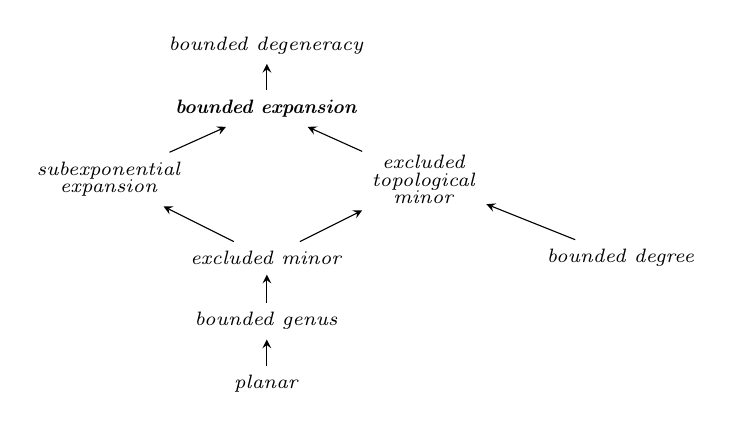
\begin{tikzpicture}

\node (bd-deg) at (11,-2.7) {\scriptsize\textit{bounded degree}};
\node[align=center] (topminor) at (8.5,-1.7) {\scriptsize\textit{excluded}\\[-2mm]\scriptsize\textit{topological}\\[-2mm] \scriptsize\textit{minor}};
\node[align=center] (sublog) at (4.5,-1.7) {\scriptsize\textit{subexponential}\\[-2mm]\scriptsize\textit{expansion}};
\node (bd-exp) at (6.5,-0.8) {\scriptsize\textbf{\textit{bounded expansion}}};
\node (degenerate) at (6.5,0) {\scriptsize\textit{bounded degeneracy}};
\node (planar) at (6.5,-4.3) {\scriptsize\textit{planar}};
\node (genus) at (6.5,-3.5) {\scriptsize\textit{bounded genus}};
\node (minor) at (6.5,-2.7) {\scriptsize\textit{excluded minor}};

%%%%%%%%%%%%%%%% Arrows %%%%%%%%%%%%%%%%

\draw[->,>=stealth] (planar) to (genus);
\draw[->,>=stealth] (genus) to (minor);
\draw[->,>=stealth] (minor) to (topminor);
\draw[->,>=stealth] (topminor) to (bd-exp);
\draw[->,>=stealth] (bd-deg) to (topminor);
\draw[->,>=stealth] (minor) to (sublog);
\draw[->,>=stealth] (sublog) to (bd-exp);
%\draw[->,>=stealth] (topminor) to[bend right=10] (bd-exp.east);
\draw[->,>=stealth] (bd-exp) to (degenerate);

\end{tikzpicture}
\end{center}
\caption{Inclusion diagram of the mentioned graph classes. }
\end{figure}\label{fig:classes}

\vspace{-3mm}
We take a step towards this goal and generalize the result of
Czygrinow et al.~\cite{czygrinow2018distributed} to classes of bounded
expansion. The notion of bounded expansion was introduced
by Ne\v{s}et\v{r}il and Ossona de Mendez~\cite{nevsetvril2008grad} and
offers an abstract definition of uniform sparseness in graphs. It is based on bounding the density of shallow minors. Intuitively, while
a minor is obtained by contracting arbitrary connected subgraphs of a graph
to new vertices, in an $r$-shallow minor we are only allowed to contract
connected subgraphs of radius at most~$r$.

A class of graphs has
bounded expansion if for every radius $r$ the set of all \mbox{$r$-shallow}
minors has edge density bounded by a constant depending only on~$r$.
We write $\nabla_r(G)$ for the maximal edge density of an
$r$-shallow minor of a graph~$G$.
Of course, every class~$\Cc$ that excludes a fixed graph $H$ as
a minor has bounded expansion. For such classes there exists an
absolute constant
$c$ such that for all $G\in\Cc$ and all~$r$
we have $\nabla_r(G)\leq c$.
Special cases are the class of
planar graphs, every class of graphs that can be drawn
with a bounded number of crossings, and every class of graphs
that embeds into a fixed surface.
Every class of intersection graphs of low density objects in low
dimensional Euclidean space has polynomial expansion, that is, the function~$\nabla_r$ is bounded polynomially in $r$ on $\Cc$. Also
every class $\Cc$ that excludes a fixed graph $H$ as
a topological minor has bounded expansion.
Important special cases are classes of
bounded degree and classes of graphs that can be drawn
with a linear number of crossings
Further examples include
classes with bounded queue-number, bounded stack-number or bounded
non-repetitive chromatic number
and the class of Erd\"os-R\'enyi random graphs with
constant average degree $d/n$, $G(n,d/n)$, has
asymptotically almost surely bounded expansion. See \cite{har2017approximation,nevsetvril2012characterisations} for all
these examples.

Hence, classes of bounded expansion are much more general than
classes excluding a topological minor. On the other hand, maybe
not surprisingly, when performing local
computations, it is not properties of minors or topological minors, but
rather of shallow minors that allow the necessary combinatorial arguments
in the algorithms. This observation was already made in the study of the kernelization complexity of dominating set on classes of sparse graphs \cite{DrangeDFKLPPRVS16,eiben2019lossy,EickmeyerGKKPRS17,FabianskiPST19,kreutzer2018polynomial}.
On the other hand, degenerate classes
are those classes where only $\nabla_0(G)$ is bounded.
These classes are hence more general than classes of bounded
expansion.

The algorithm of Czygrinow et al.~\cite{czygrinow2018distributed} is
based on an quite complicated iterative process of choosing dominating
vertices from so called
\emph{pseudo-covers}. Based on the fact that classes with excluded topological minors in particular exclude some complete bipartite graph
$K_{t,t}$ as a subgraph it is proved that this iterative process terminates
after at most $t$ rounds and
produces a good approximation of a minimum dominating set.

In this paper we make three contributions. First, we simplify the
arguments used by Czygrinow et al.\ and give a much more accessible
description of their algorithm. Second, we identify the property that $\nabla_1(G)$ is
bounded by a constant as the key property that makes the algorithm
work. Classes with only this restriction are
even more general than bounded expansion classes, hence, we generalize
the algorithm to the most general classes on which it (and similar
approaches based on covers or pseudo-covers)
can work. We demonstrate that the pseudo-covering method cannot
be extended e.g.\ to classes of bounded degeneracy. Finally,
Czygrinow et al.\ explicitly stated that they did not aim to
optimize any constants, and as presented, the constants in their
construction are enormous. We optimize the bounds that arise in
the algorithm in terms of $\nabla_1(G)$.
%\textcolor{red}{We demonstrate
%the improvements in particular in the case of planar graphs. We show
%that the algorithm provides the best known approximation on
%planar graphs. The approximation ratio seems to be
%$2+3\cdot 7+9=33$. The best currently known bounds are $52$.
%This will be bigger because we need the neighborhoods to be
%larger than $k^t(2t+tK)$... Check this.}
%\sebi{If we have not enough time we drop the planar case.}
Even though the constants
are still large, they are by magnitudes smaller than those in the
original presentation.

\begin{theorem}
There exists a LOCAL algorithm that for any given graph $G$ and
an upper bound on $\nabla_1(G)$ as input
computes in a constant number of rounds a dominating set
of size $\mathcal{O}(\nabla_1(G)^{4t\nabla_1(G)+t})\cdot \gamma(G)$,
where $t\leq 2\nabla_1(G)+1$ is minimum such that $K_{t,t}\not\subseteq G$.
\end{theorem}

\pagebreak
Before we go into the technical details let us give an overview of the
algorithm. The algorithm works in three steps, in each step ($i\in \{1,2,3\}$) computing a small set $D_i$ that is added to the dominating set.

\begin{enumerate}
\item Compute the set $D_1$ of all $v$ such that $N(v)$ cannot be
dominated by a small number (the constant $2\nabla_1(G)$) of vertices different from $v$.
Remove~$D_1$ from~$G$ and mark all its neighbors as dominated.
The fact that $|D_1|$ is linearly bounded in~$\gamma(G)$ goes back to work
of~\cite{lenzen2013distributed} and we prove our bounds in \cref{lem:neighborhood-dom1}.
\item In parallel for every vertex $v=v_1$ we compute all so called
\emph{domination sequences $v_1,\ldots, v_s$}, defined formally
in \cref{def:dom-sequence}. This step is based on the construction of
pseudo-covers as in the work of Czygrinow et al.~\cite{czygrinow2018distributed}.
We add all vertices $v_s$ to the set
$D_2$. We prove that this set is small compared to~$\gamma(G)$ in \cref{lem:small-D-hat}. Remove $D_2$ from $G$ and mark its neighbors as
dominated.
\item All remaining vertices have small degree, as proved in \cref{crl:d3}, and hence
in a final step we can add all non-dominated vertices to a set $D_3$. We finally
return the set $D_1\cup D_2\cup D_3$.
\end{enumerate}

The main
open question that remains in this line of research is whether we can
compute constant factor approximations of minimum dominating sets
in a constant number of rounds in classes of bounded degeneracy.

% !TEX root = sirocco-main.tex

\section{Preliminaries}

In this section we fix our notation and prove some basic lemmas
required for the algorithm. We use standard notation from graph
theory and refer to the literature for extensive background. For an
undirected and simple graph~$G$ we denote by $V(G)$
the vertex set and by $E(G)$ the edge set of $G$. We also refer
to the literature, for the
formal definition of the LOCAL model of distributed computing.

A graph~$H$ is a minor of a graph~$G$, written~$H\minor G$, if
there is a set \mbox{$\{G_v :v\in V(H)\}$} of pairwise vertex disjoint and
connected subgraphs
$G_v\subseteq G$ such that if~$\{u,v\}\in E(H)$, then there is an edge
between a vertex of~$G_u$ and a vertex of~$G_v$. We call $V(G_v)$ the
\emph{branch set} of $v$ and say that it is
\emph{contracted} to the vertex~$v$.
%If $G_1,\ldots, G_k\subseteq V(G)$
%are pairwise vertex disjoint and connected subgraphs of $G$, then we write
%$G/G_1/\ldots/G_k$ for the minor obtained by contracting the subgraphs~$G_i$ (observe that the order of contraction does not matter as the
%$G_i$'s are vertex disjoint).

For a non-negative integer~$r$, a graph
$H$ is an \emph{$r$-shallow minor} of $G$, written
$H\minor_r G$, if there is a set~$\{G_v : v\in V(H)\}$ of pairwise
vertex disjoint connected subgraphs
$G_v\subseteq G$ of radius at most $r$ such that if~$\{u,v\}\in E(H)$,
then there is an edge between a vertex of~$G_u$ and a vertex of~$G_v$.
Observe that a $0$-shallow minor of $G$ is just a subgraph of $G$.

We write $\nabla_r(G)$ for $\max_{H\minor_r G}|E(H)|/|V(H)|$. Observe
that $\nabla_0(G)$ denotes the maximum average edge density of $G$
and $2\nabla_0(G)$ bounds the degeneracy of~$G$, which is defined
as $\max_{H\subseteq G}\delta(H)$. Here, $\delta(H)$ denotes
the minimum degree of~$H$.
%
A class~$\Cc$ of graphs has \emph{bounded expansion} if there is a function
$f:\N\rightarrow\N$ such that $\nabla_r(G)\leq f(r)$ for all graphs $G\in \Cc$.
This is equivalent to demanding that the degeneracy of each $r$-shallow minor
of $G$ is functionally bounded by~$r$.

We write~$K_{s,t}$ for the complete bipartite
graph with partitions of size~$s$ and~$t$, respectively. Observe that
$K_{t,t}$ has $2t$ vertices and $t^2$ edges, hence, if
\mbox{$\nabla_0(G)< t/2$}, then $G$ excludes $K_{t,t}$ as a subgraph.

For a graph $G$ and $v\in V(G)$ we write $N(v)=\{w~:~\{v,w\}\in E(G)\}$
for the \emph{open neighborhood} of $v$ and $N[v]=N(v)\cup\{v\}$ for
the \emph{closed neighborhood} of~$v$. For a set $A\subseteq V(G)$ let
$N[A]=\bigcup_{v\in A}N[v]$. We write $N_r[v]$ for the set
of vertices at distance at most $r$ from a vertex $v$.
A dominating set in a graph~$G$ is a set
$D\subseteq V(G)$ such that $N[D]=V(G)$. We write $\gamma(G)$ for
the size of a minimum dominating set of $G$. For $W\subseteq V(G)$
we say that a set $Z\subseteq V(G)$ \emph{dominates} or \emph{covers} or
is a \emph{cover} of $W$ if $W\subseteq N[Z]$.
Observe that we do not
require $Z\cap W=\emptyset$ as Czygrinow et al.\ do for covers.

\smallskip
The following lemma is one of the key lemmas used for the algorithm. It goes back to~\cite{lenzen2013distributed}.

\begin{lemma}\label{lem:neighborhood-dom1}
Let $G$ be a graph. Then there are less than $2\gamma(G)$ vertices $v$ with the property that $N(v)$ cannot be dominated by at most $2\nabla_1(G)$ vertices different from $v$.
\end{lemma}
\begin{proof}
Let $\gamma=\gamma(G)$ and $\nabla_1=\nabla_1(G)$ and assume that there are $2\gamma$ such vertices $a_1,\ldots,a_{2\gamma}$. We proceed towards a contradiction.
  Let $\{d_1,\ldots,d_\gamma\}$ be a minimum dominating set. At least $\gamma$ of the $a_i$'s are not in this dominating set. We can hence assume w.l.o.g.~that $\{a_1,\ldots,a_{\gamma}\}$ and $\{d_1,\ldots,d_\gamma\}$ are two disjoint sets of vertices.

We build a $1$-shallow minor $H$ of the graph $G$ with the following $2\gamma$ branch sets. For every $i\le \gamma$, we have a branch set
$A_i=\{a_i\}$ and a branch set $D_i=N[d_i]\setminus (\{a_1,\ldots, a_\gamma\}\cup \bigcup_{j<i}N[d_j] \cup \{d_{i+1},\ldots, d_\gamma\})$.
We call the associated vertices of $H$ $a_1',\ldots, a_\gamma',d_1',\ldots,
d_\gamma'$.

Since $\{d_1,\ldots, d_\gamma\}$ is a dominating set of $G$ and by assumption on $N(a_i)$, we have that in $H$, every $a'_i$ is connected to at least $2\nabla_1+1$ of the $d'_i$.
  We therefore have that $|V_H|=2\gamma$ and $|E_H| \ge \gamma(2\nabla_1+1)$, hence $|E_H|> |V_H|\nabla_1$, a~contradiction.
\end{proof}

Note that we cannot locally determine the number $\nabla_1(G)$.
We must hence assume that it is given with the input. Observe that
similarly, the algorithm of Czygrinow et al.\ works with the assumption
that the input excludes a complete graph with $t$ vertices as a topological
minor. This implies a bound on the edge density of topological minors
in $G$, which can be seen as being given with the input.

The algorithm proceeds in three phases. The first phase is
based on \cref{lem:neighborhood-dom1} as follows.
In the LOCAL model we can learn the distance-$2$
neighborhood~$N_2[v]$ of every vertex $v$ in $2$ rounds,
and then locally check
whether~$N(v)$ can be domi\-nated by at most $2\nabla_1(G)$
vertices.

\begin{tcolorbox}
% \fbox{
% \begin{minipage}{0.9\linewidth}
We let $D_1$ be the set of all vertices that do not have this
property. By \cref{lem:neighborhood-dom1}
we have $|D_1|\leq 2\gamma(G)$. We remove $D_1$ from the
graph and mark all its neighbors as dominated in one additional round.
% \end{minipage}
% }
\end{tcolorbox}


In the following we fix a graph $G$ and we assume that $N(v)$ can be
dominating by at most $2\nabla_1(G)$ vertices different from $v$
for all $v\in V(G)$. We write $\nabla_1$ for~$\nabla_1(G)$ and
we let $t\leq 2\nabla_0(G)+1$ be the smallest positive integer
 such that~$G$ excludes
$K_{t,t}$ as a subgraph. Note that this number is not required
as part of the input. We let $k\coloneq 2\nabla_1$.

\begin{example}
  A planar $n$-vertex graph has at most $3n-6$ edges. A minor of a
  planar graph is again planar, hence for planar graphs $G$ we have $\nabla_r(G) \leq 3$ for all $r\geq 0$ and $k=2\nabla_1(G)\leq 6$.
\end{example}

We also fix a minimum dominating set $D$ of $G$
of size~$\gamma$.
% In the following, when we speak of ``almost all vertices'', we mean all but at most~$c\gamma$ vertices for some
% constant $c$. This is again motivated by the argument that adding
% any~$c\gamma$ vertices
% to the dominating set will still give a constant factor approximation.
The following lemma is proved exactly as \cref{lem:neighborhood-dom1}.

\begin{lemma}\label{lem:neighborhood-dom2}
There are less than $2\gamma$ vertices $v$ with the property
that $N(v)$ cannot be dominated by at most $2\nabla_1$ vertices
from $D$ and different from $v$.
\end{lemma}

Unfortunately, we cannot determine these vertices locally, as it requires
know\-ledge of $D$, however, this structural property is very useful for
our further argumentation.

\begin{tcolorbox}
% \begin{minipage}{0.92\linewidth}
Denote by $\hat D$ the set of all vertices $v$
whose neighborhood cannot be dominated
by $2\nabla_1$ vertices of $D$ different from $v$.
Let $D'=D\cup \hat D$.
% \end{minipage}
\end{tcolorbox}

According to %\cref{lem:neighborhood-dom1} and
\cref{lem:neighborhood-dom2}, $D'$ contains at most
%$(1+4\nabla_1)\gamma$ vertices.
$3\gamma$ vertices.
% \alex{shouldn't we simply add $v$ in $D'$? We then get that $|D'|\le 3\gamma$.\\
%   $\gamma$ for $D$, and at most $2\gamma$ such vertices.}
Let us stress that~$D'$ will never be computed by our LOCAL algorithm. We only use
its existence in the correctness proofs.

\smallskip
We can apply these
lemmas to obtain a constant factor approximation for a dominating
set only if $\nabla_1(G)$ is bounded by a constant. For example in graphs of bounded degeneracy in general the number of vertices that dominate the
neighborhood of a vertex can only be bounded by $\gamma(G)$.
Hence, the approach based on covers and pseudo-covers that is employed
in the following cannot be extended to degenerate  graph classes.

\begin{example}
Let $G(\gamma,m)$ be the graph with vertices $v_i$ for $1\leq i\leq \gamma$,
$w^j$ for $1\leq j\leq m$ and $s_i^j$ for $1\leq i\leq \gamma, 1\leq j\leq m$.
We have the edges $\{v_1, w^j\}$ for $1\leq j\leq m$, hence $v_1$
dominates all $w^j$. We have the edges $\{w^j, s_i^j\}$ for all $1\leq i\leq \gamma,
1\leq j\leq m$, hence, the $s_i^j$ are neighbors of $w^j$. Finally,
we have the edges $\{v_i, s_i^j\}$, that is, $v_i$ dominates the $i$th
neighbor of $w_j$. Hence, for $m>\gamma$,
$G(\gamma, m)$ has a dominating set of size
$\gamma$ and $m$ vertices whose neighborhood can be dominated
only by $\gamma(G)$ vertices. \cref{lem:neighborhood-dom1} implies
that $\gamma < 2\nabla_1$, and as we can choose~$m$ arbitrary
large, we cannot usefully apply \cref{lem:neighborhood-dom1}.
Furthermore, $G(\gamma,m)$ is
\mbox{$2$-degenerate}, showing that these methods cannot be applied on
degenerate graph classes.

\begin{center}
  \begin{figure}
    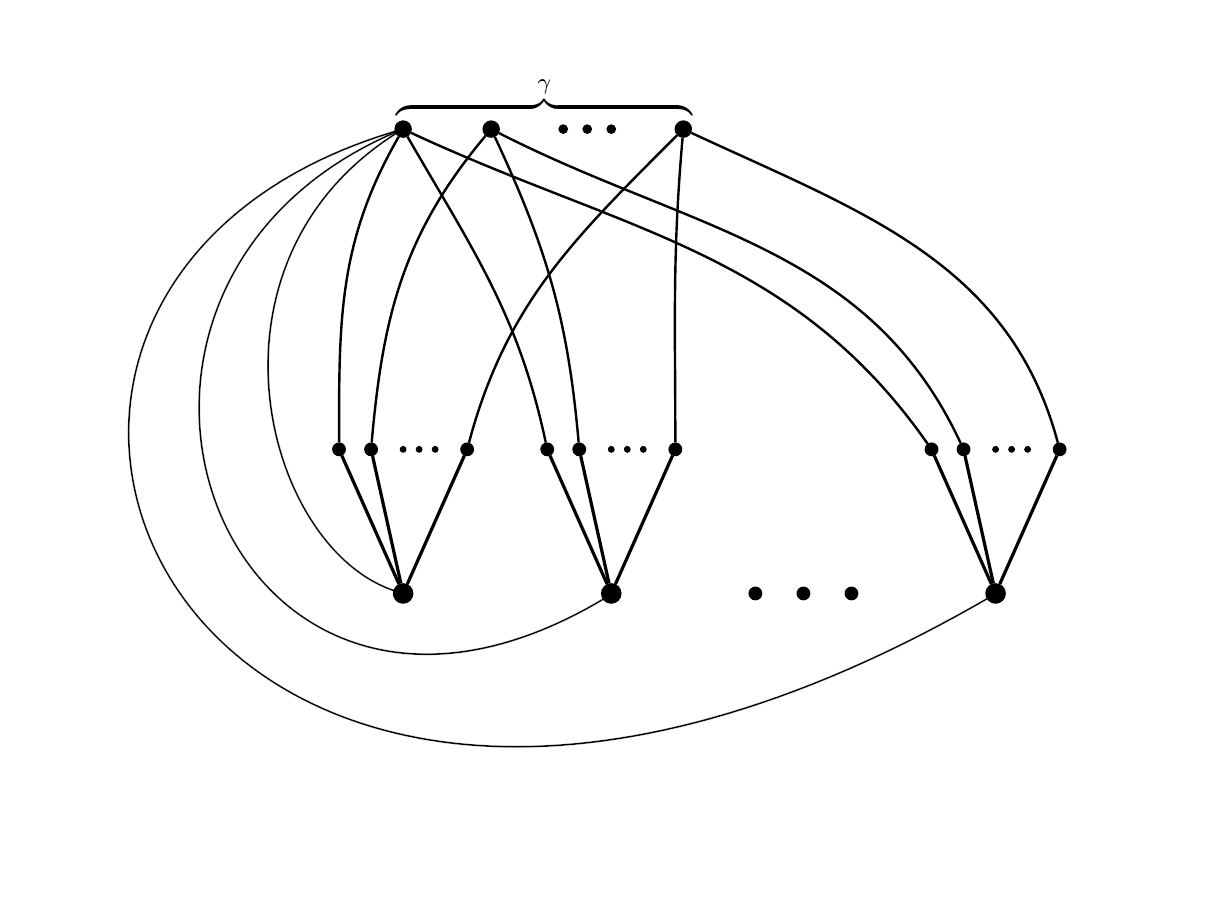
\includegraphics[scale=0.3]{ds1.png}
    \caption{ A $2$-degenerate graph where for many $v\in V(G)$ the set $N(v)$ can only be dominated by at least $\gamma$ vertices different from $v$. }
  \end{figure}
\end{center}
\end{example}

% !TEX root = sirocco-main.tex

\section{Covers and pseudo-covers}

Intuitively, the vertices from a cover of a set $W$ can
take different roles. A few vertices of a cover may cover almost the
complete set $W$, while a few others are only there to cover what was
left over. The key observation of Czygrinow et al.\ is that in classes that
exclude some~$K_{t,t}$ as a subgraph, there can only be few of such
high degree covering vertices, while there can be arbitrarily many vertices
that cover at most $t-1$ vertices of~$W$ (the same vertices can be covered
over and over again). This observation can be applied recursively and is
distilled into the following two definitions. Recall that by the processing
carried out in the first phase of the algorithm
we know that every neighborhood $N(v)$ can be covered by $k=2\nabla_1$ vertices different from $v$.
% For the rest of this article we fix
% $\alpha\coloneqq 1/k$, $\ell=8\nabla_1/\alpha^2+1=4k^3+1$ and $q=4k^4$.
% These constants will be needed in the following definitions of pseudo-covers
% and domination sequences.
We recall all fixed parameters for easy to find reference.

\bigskip
\begin{tcolorbox}
\begin{tabular}{l l}
- $G$ & :~ fixed graph. \\
- $\gamma$ & :~ $\gamma(G)$.\\
- $\nabla_1$ & :~ $\nabla_1(G)$. \\
- $t$ & :~ smallest integer such that $G$
excludes $K_{t,t}$ as a subgraph\\
- $D_1$ & :~ defined and computed in \cref{lem:neighborhood-dom1}.\\
- $D$ & :~ fixed dominating set of $G$ of size $\gamma$ (not computed).\\
- $\hat{D}$ & :~ defined in \cref{lem:neighborhood-dom2} (not computed).\\
- $D'$ & :~ $D \cup \hat{D}$ (not computed).
\end{tabular}
\end{tcolorbox}

% For the rest of this article we fix
% $\alpha\coloneqq 1/k$, $\ell=8\nabla_1/\alpha^2+1=4k^3+1$ and $q=4k^4$.
% These constants will be needed in the following definitions of pseudo-covers
% and domination sequences.
% We also fix the following constants to follow the presentation
% of~\cite{czygrinow2018distributed}.

Following the presentation of~\cite{czygrinow2018distributed}, we name and fix
these constants for the rest of this article.

\begin{tcolorbox}
\begin{tabular}{l l}
- $k$       & $\coloneqq~ 2\nabla_1$.\\
- $\alpha$  & $\coloneqq~ 1/k$.\\
- $\ell$    & $\coloneqq~ 8\nabla_1/\alpha^2+1=4k^3+1$.\\
- $q$       & $\coloneqq~ 4k^4$.
\end{tabular}
\end{tcolorbox}


\begin{definition}
A vertex $z\in V(G)$ is \emph{$\alpha$-strong} for a vertex set $W\subseteq V(G)$ if $|N[z]\cap W|\geq \alpha|W|$.
\end{definition}

The following is the key definition by Czygrinow et al.~\cite{czygrinow2018distributed}.

\begin{definition}
A \emph{pseudo-cover} (with parameters $\alpha, \ell, q, k$)
of a set $W\subseteq V(G)$ is a
sequence $(v_1,\ldots, v_m)$ of vertices
such that  for every $i$ we have
\begin{itemize}
\item $|W\setminus \bigcup_{j\le m}N[v_j]|\leq q$,
\item $v_i$ is $\alpha$-strong for $W\setminus\bigcup_{j<i}N[v_j]$,
\item $|N[v_i]\cap (W\setminus\bigcup_{j<i} N[v_j])|\geq \ell$,
\item $m\leq k$.
\end{itemize}
\end{definition}
Intuitively, all but at most $q$ elements of the set $W$ are covered by the $(v_i)_{i\le m}$.
Additionally, each element of the pseudo-cover dominates both an
$\alpha$-fraction of what remains to be dominated, and at least $\ell$ elements.
Note that with our choice of constants, if there are more than $q$ vertices not
covered yet, any vertex that covers an $\alpha$-fraction of what remains also
covers at least $\ell$ elements.


The next lemma shows how to derive the existence of pseudo-covers from
the existence of covers.

\begin{lemma}\label{lem:cover-to-pseudo-cover}
Let $W\subseteq V(G)$ be of size at least
$q$ and let~$Z$ be a cover of $W$ with~$k$ elements.
There exists an ordering of the vertices of $Z$ as $z_1,\ldots, z_k$
and $m\leq k$ such that $(z_1,\ldots, z_m)$ is a pseudo-cover of $W$.
\end{lemma}
\begin{proof}
 We build the order greedily by induction. We order the elements by neighborhood size, while removing the neighborhoods of the previously ordered vertices. More precisely, assume that $(z_1,\ldots,z_i)$ have been defined for \mbox{some~$i\ge 0$}. We then define $z_{i+1}$ as the element that maximizes $|N[z] \cap (W \setminus \bigcup_{j\le i}N[z_j])|$.

 Once we have ordered all vertices of $Z$, we define $m$ as the maximal integer not larger than $k$ such that for every $i \le m$ we have:
 \begin{itemize}
   \item $z_i$ is $\alpha$-strong for $W\setminus\bigcup_{j<i}N[z_j]$, and
   \item $|N[z_i] \cap (W \setminus \bigcup_{j\le i}N[z_j])| \ge \ell$.
 \end{itemize}

This made sure that $(z_1,\ldots, z_m)$ satisfies the last 3 properties of a
 pseudo-cover of $W$. It only remains to check the first one.
 To do so, we define $W' \coloneq W \setminus\bigcup_{i\le m}N[z_i]$. We want to prove
 that $|W'| \le q$. Note that because $Z$ covers~$W$, if $m=k$ we
 have $W'=\emptyset$ and we are done. We can therefore assume
 that $m<k$ and $W'\neq \emptyset$. Since $Z$ is a cover of $W$,
 we also know that $(z_{m+1},\ldots z_k)$ is a cover of $W'$,
 therefore there is an element in $(z_{m+1},\ldots z_k)$ that
 dominates at least a $1 / k$ fraction of $W'$. Thanks to the
 previously defined order, we know that~$z_{m+1}$ is such element.
 Since $\alpha = 1/k$, it follows that~$z_{m+1}$ is $\alpha$-strong
 for $W'$.
 This, together with the definition of $m$, we have that $|N[z_i] \cap (W \setminus \bigcup_{j\le i}N[z_j])| < \ell$ meaning that $|N[z_{m+1}] \cap W'| < \ell$. This implies that $|W'|/k < \ell$. And since $\ell = q/k$, we have $|W'|<q$.
%
  Hence, $(z_1,\ldots, z_m)$ is a pseudo-cover of $W$.
\end{proof}

%We will apply the pseudo-covers to neighborhoods
%of vertices.

While there can exist unboundedly many covers for a set $W\subseteq V(G)$,
the nice observation of Czygrinow et al.\ was that the number of
pseudo-covers is bounded whenever the input graph excludes some
biclique $K_{s,t}$ as a subgraph. We do not state the result in this
generality, as it leads to enormous constants. Instead, we focus on the
case where small covers exist, that is, on the case where~$\nabla_1(G)$
is bounded and optimize the constants for this case.

\begin{lemma}\label{lem:num-high-degree}
Let $W\subseteq V(G)$ of size at least $8\nabla_1 / \alpha^2$.
Then there are at most $4\nabla_1/\alpha$ vertices that are
$\alpha$-strong for $W$.
\end{lemma}
\begin{proof}
  Assume that there is such a set $W$ with at least $c\coloneq 4\nabla_1 /\alpha$ vertices that are $\alpha$-strong for $W$.
  We build a $1$-shallow minor $H$ of the graph $G$ with $|W|$ branch sets.
  Each branch set is either a single element of $W$, or a pair $\{w,a\}$, where $w$ is in $W$ and $a$ is an $\alpha$-strong vertex for $W$, connected to $w$, and that is not in $W$. This is obtained by iteratively contracting one edge of an $\alpha$-strong vertex with a vertex of $W$. This is possible because $\alpha |W|>c$, so during the process and for any \mbox{$\alpha$-strong} vertex we can find a connected vertex in $W$ that is not part of any contraction.

  Once this is done, we have that $|V_H|=|W|$. For the edges, each of the \mbox{$\alpha$}-strong vertices can account for $\alpha |W|$ many edges. We need to subtract~$c^2$ from the total as we do not count twice an edge between two strong vertices. Therefore $|E_H| \ge c\alpha |W| - c^2$. Note also that because $|W| \ge 8\nabla_1 / \alpha^2$, we have that $ 2\nabla_1\ge (4\nabla_1)^2 / (\alpha^2|W|)$. All of this together leads to:

  $$\frac{|E_H|}{|V_H|} \ge \frac{c\alpha |W| - c^2}{|W|} \ge 4 \nabla_1 - \frac{(4\nabla_1)^2}{\alpha^2|W|} \ge 4\nabla_1 - 2\nabla_1 > \nabla_1 $$

  This contradicts the definition of $\nabla_1$.
\end{proof}

This leads quickly to a bound on the number of pseudo-covers.

\begin{lemma}\label{lem:num-pseudo-covers}
For every $W\subseteq V(G)$ of size at least $\ell$, the number of pseudo-covers is bounded by $2(4\nabla_1(G)/\alpha)^k$.
\end{lemma}

The proof of the lemma is exactly as the proof of Lemma~7 in the
presentation of Czygrinow et al.~\cite{czygrinow2018distributed},
we therefore refrain from repeating it here.

%
%Having previous decided to fix $K$ and $\alpha$, \cref{lem:num-pseudo-covers}
%yields the following handy corollary.
%\begin{corollary}\label{cor:num-pseudo-covers}
%  Let $G$ be a graph. Fixe $k\coloneq 2\nabla_1(G)$, and then define
%  $\alpha = 1/k$, $K=k$, $\ell =4k^3+1$, and $q:= 4k^4$.
%  Then for every $W\subseteq V(G)$ of size at least $\ell$, the number of
%  $(\alpha,q,\ell,K)$-pseudo-covers of $W$
%  is bounded by $2(2k^2)^k$.
%\end{corollary}

% \textcolor{blue}{
% \begin{example} Let $G$ be a planar graph. We can strongly optimize
% the construction. For $\alpha>0, \ell\geq 8, q\geq 0$ and
% $K\leq 6$ the number of vertices appearing in any $(\alpha, q,\ell, K)$-pseudo-cover
% of $N(v)$ for a vertex $v$ is at most $7$.
% The neighborhood $N(v)$ is dominated by $v$ and also by
% at most $6$ vertices from $D'$. Then there does not exist
% a further vertex that dominates at least $8$ vertices of
% $N(v)$ as $G$ is planar. PROOF+PICTURE.
% \end{example}
% }

\begin{tcolorbox}
We write $\Tt(v)$ for the set of all pseudo-covers
of $N(v)$ and $\Pp(v)$ for the set of all vertices that appear in a
pseudo-cover of $N(v)$.
\end{tcolorbox}



\begin{corollary}\label{cor:nb-dominators}
For every $v\in V(G)$ with $|N(v)|> \ell$, we have
  $|\Tt(v)|\le 2(2k^2)^k$ and $|\Pp(v)|\le 2k(2k^2)^k\le (2k)^{2k+1}$.
\end{corollary}

% !TEX root = sirocco-main.tex

\section{Finding dominators}


Recall that by \cref{lem:neighborhood-dom2} for every $v\in V(G)$ we can
cover $N(v)$ with at most~$k$ vertices from $D'$.
To first gain an intuitive understanding of the second phase of the
algorithm, where we construct a set $D_2\subseteq V(G)$, let us consider the
following iterative procedure.

Fix some $v\in V(G)$. Let $v_1=v$ and $B_1\coloneqq N(v)$
and assume $|B_1|\geq k^{t-1}(2t{-}1)$. We consider $s$
vertices $v_1,v_2\ldots, v_s$ as follows.
Choose as~$v_2$ an arbitrary vertex different from $v_1$
that dominates at least $k^{t-2}(2t-1)$ vertices of~$B_1$, that is,
a vertex that satisfies $|N[v_2]\cap B_1|\geq k^{t-2}(2t-1)$.
Note that any vertex~$v_2$ that dominate a $1/k$-fraction of $B_1$ can
be such vertex, i.e.~it is enough for $v_2$ to be $\alpha$-strong for $B_1$.

Let $B_2\coloneqq N(v_2)\cap B_1$. Observe that we consider
the open neighborhood of $v_2$ here, hence $B_2$ does
not contain $v_2$. Hence, $|B_2|\geq k^{t-2}(2t-1)-1\geq
k^{t-2}(2t-2)$.
We continue to choose vertices $v_3,\ldots$ inductively
just as above. That is, if the vertices $v_1,\ldots,v_i$ and sets
$B_1,\ldots, B_i\subseteq V(G)$ have been defined, we choose
the next vertex $v_{i+1}$ as an arbitrary vertex not in $\{v_1,\ldots,
v_i\}$ that dominates
at least $k^{t-i-1}(2t-i)$ vertices of $B_i$, that is, a vertex with
$|N[v_{i+1}]\cap B_i| \ge k^{t-i-1}(2t-i)$ and let
$B_{i+1}\coloneqq N(v_{i+1})\cap B_i$, of size at least
$k^{t-i-1}(2t-i-1)$.



\begin{lemma}\label{lem:sequence}
Assume $|N(v)|\geq k^{t-1}\cdot (2t-1)$. Let $v_1,\ldots, v_s$
be a maximal sequence obtained as above. Then $s<t$ and
$D'\cap \{v_1,\ldots, v_s\}\neq \emptyset$.
\end{lemma}
\begin{proof}
  Assume that we can compute a sequence $v_1,v_2,\ldots,v_t$. By definition,
  every $v_i$ is connected to every vertices of $B_t$.
  For every $1\leq i\leq t$ we have $|B_i|\geq k^{t-i}(2t-i)$
  and therefore
  $|B_t|\ge t$. This shows that the two sets
  $\{v_1,\ldots,v_t\}$ and $B_t$ form a $K_{t,t}$ as a subgraph of $G$.
  Since this is not possible, the process must stop having performed at
  most $t-1$ rounds.

  We now turn to the second claim of the lemma. Assume that
  $v_1,v_2,\ldots,v_s$ is a maximal sequence for some $s < t$. We assume
  $v_1\not\in \hat{D}$, otherwise, we are done, as $\hat{D}\subseteq D'$.
  Because $s <t$,
  we have that $B_s$ is not empty. Because $B_s \subseteq B_1 = N(v_1)$, we have
  that $B_s$ can be dominated with at most~$k$ elements of~$D$ (by definition of $\hat{D}$), and in particular by at most $k$ elements of $D'$. Therefore,
  there must be an element~$v$ of~$D'$ that dominates a $1/k$ fraction of $B_s$.
  If $v$ was not one of the $v_1,\ldots,v_s$, we could have continued the
  sequence by defining $v_{s+1} \coloneqq v$.
  Since the sequence is maximal, $v$ must be one of the $v_1,\ldots,v_s$,
  which leads to $D'\cap \{v_1,\ldots, v_s\}\neq\emptyset$.

%
%  By assumption, $B_1$ is dominated by at most $k$
%  vertices of $D'$. Hence, unless $v_1$ is in $B'$, we can find
%  a vertex $v_2\in V(G)$ that dominates at least
%  a $1/k$ fraction of $B_1$, that is, at least $k^{t-1}\cdot 2t$ vertices
%  of $B_1$. Let $B_2\coloneqq N(v_2)\cap B_1$,
%  hence $|B_2|\geq k^{t-1}\cdot 2t-1\geq k^{t-1}\cdot (2t-1)$.
%  Observe that we subtracted $1$, as $v_2$ is not in $B_2$.
%
%  Assume that neither $v_1$ nor $v_2$ are in $D'$. We repeat the same argument
%  as above for $B_2$. Because $B_2$ is dominated by at most $k$ vertices
%  of $D'$, there exists a vertex $v_3\in V(G)$ that
%  dominates at least a $1/k$ fraction of $B_2$, that is, at least
%  $k^{t-2}\cdot (2t-1)$ vertices of~$B_2$. Let $B_3\coloneqq
%  (N(v_3)\cap B_2)$,
%  hence $|B_3|\geq k^{t-2}\cdot (2t-1)-1\geq k^{t-2}\cdot (2t-2)$.
%  We repeat the argument for $v_4,\ldots,v_{\ell}$ and $B_4,\ldots, B_{\ell}$, each $B_i$
%  for $1\leq i\leq \ell<t$ of size at
%  least $k^{t-i}\cdot (2t-i)$, ending with a set~$B_{\ell}$ of
%  size at least $k\cdot (t+1)$.
%
%  Hence, assuming that $v_1,\ldots, v_\ell\not\in D'$, we have $\ell=t-1$
%  and there must
%  exist a vertex~$v$ with
%  $|N(v)\cap B_\ell|\geq t+1$. Fix any subset $B=\{w_1,\ldots, w_t\}$
%  of $N(v)\cap B_\ell$ of size exactly $t$. Then the vertices
%  $v,v_1,\ldots, v_{t-1}$ and the vertices $w_1,\ldots, w_t$
%  form a subgraph $K_{t,t}$, contradicting that
%  such a subgraph does not exist in $G$. Hence, one of
%  $v_1,\ldots, v_\ell$ must be contained in $D'$.
\end{proof}

We aim to carry out this iterative process in parallel
for all vertices \mbox{$v\in V(G)$} with a sufficiently large neighborhood.
Of course, in the process
we cannot tell when we have encountered the element of~$D'$.
Hence, from the constructed vertices $v_1,\ldots, v_s$
we will simply choose the element~$v_s$ into the dominating set.
Unfortunately, this approach alone can give us arbitrarily large
dominating sets, as we can have many choices for the vertices
$v_i$, while already $v_1$ was possibly optimal.
We address this issue by restricting
the possible choices for the vertices~$v_i$.

\begin{definition}\label{def:dom-sequence}
  For any vertex $v\in V(G)$, a {\em $k$-dominating-sequence} of $v$ is a sequence
  $(v_1,\ldots,v_s)$ for which we can define sets $B_1,\ldots,B_s$ such that:
  \begin{itemize}
    \item $v_1=v$, $B_1 \subseteq N(v_1)$,
    \item for every $i\le s$ we have $B_{i} \subseteq N(v_{i})\cap B_{i-1}$,
    \item $|B_{i}|\geq k^{t-i}(2t-i+(t-i)q)$
    \item and for every $i\le s$ we have $v_i\in \Pp(v_{i-1})$.
  \end{itemize}
  A $k$-dominating-sequence $(v_1,\ldots,v_s)$ is {\em maximal} if there is no
  vertex $u$ such that $(v_1,\ldots,v_s,u)$ is a $k$-dominating-sequence.
\end{definition}

%Remember that $t$ is an integer such that $G$ excludes a $K_{t,t}$ subgraph,
%and that $2\nabla_0(G)+1$ is such an integer. Also remember that we
%defined $K=k$,
%$\alpha = 1/k$, $\ell = 4k^3$ and $q=4k^4$, where $k=2\nabla_1(G)$.
Note that this definition requires $|N(v)|\ge k^{t-1}(2t-1+(t-1)q)$. For a
vertex~$v$ with a not sufficiently large neighborhood, there are no
$k$-dominating-sequences of $v$.
We show two main properties of these dominating-sequences.
First, \cref{lem:max-dom-sequence} shows that a maximal dominating sequence must
encounter $D'$ at some point. Second, with \cref{lem:shape-sequences,lem:small-D-hat,lem:inclusion-D-hat},
we show that collecting all ``end points'' of all maximal dominating sequences
results in a set $D_2$ of size linear in the size of $D'$. While $D'$ cannot be computed, we
can compute $D_2$.
%
% For $v\in V(G)$ consider the following modified construction of
% $v_1,\ldots, v_s$. Every $v_i$ is chosen such that it has
% an intersection $|N(v_i)\cap B_{i-1}|\geq k^{t-i}(2t-i+(t-i)q)$.
% Furthermore, we
% restrict the choice of $v_i$ to the set of vertices that appear
% in some $(\alpha,q,\ell,K)$-pseudo-cover in $\Tt(v_{i-1})$.
% We observe that this process still works as desired.

\begin{lemma}\label{lem:max-dom-sequence}
Let $v$ be a vertex %with $|N(v)|\geq k^{t-1}\cdot (2t-1+(t-1)q)$,
and let
$(v_1,\ldots, v_s)$ be a maximal $k$-dominating-sequence of $v$. Then $s<t$ and
$D'\cap \{v_1,\ldots, v_s\}\neq \emptyset$.
\end{lemma}
\begin{proof}
  The statement $s<t$ is proved exactly as for \cref{lem:sequence}.\\
  To prove the second statement we assume, in order to reach
  a contradiction, that $D'\cap\{ v_1,\ldots, v_s\}=\emptyset$.
  We have that $B_s \subseteq N(v_s)$, and remember that $N(v_s)$ can be
  dominated by at most $k$ elements of $D'$. By \cref{lem:cover-to-pseudo-cover},
  we can derive a pseudo-cover $S=(u_1,\ldots,u_m)$ of
  $N(v_s)$, where $m\le k$ and every $u_i$ is an element of $D'$.
  Let $X$ denote the set (of size at most $q$) of vertices not covered by $S$.
  As $S$ contains at most $k$ vertices there must exist a
  vertex $u$ in~$S$ that covers at least a $1/k$ fraction of
  $B_s\setminus X$.
  By construction, we have that $|B_s| \ge k^{t-s}\cdot(2t-s+(t-s)q)\ge k(t+q)$
  because $s<t$. Therefore $|B_s\setminus X| \ge k$ and we have
  $$|N[u]\cap B_{s}|\geq \frac{|B_s|-q}{k}
  \geq\frac{k^{t-s}(2t-s+(t-s)q) -q}{k},$$
  hence
  $$|N[u]\cap B_{s}| \geq\frac{k^{t-s}(2t-s+(t-s-1)q)}{k} \geq k^{t-s-1}(2t-s+(t-s-1)q),$$
  and therefore
  $$ |N(u)\cap B_{s}| \geq |N[u]\cap B_{s}|-1 \geq k^{t-s-1}(2t-s-1+(t-s-1)q).$$
  So we can continue the sequence $(v_1,\ldots,v_s)$ by defining
  $v_{s+1}\coloneqq u$. In conclusion if $(v_1,\ldots,v_s)$ is a maximal
  sequence, it contains an element of $D'$.
%  \alex{end of the proof}
%The statement $s<t$ is proved exactly as above. To show that
%$D'\cap \{v_1,\ldots, v_s\}\neq
%\emptyset$ holds, we show that in each step $i>1$ we have the
%possibility of choosing some vertex that appears in some
%$(\alpha,q,\ell,k)$-pseudo-cover $S\in \Tt(v_{i-1})$.
%As $B_i\subseteq N(v_{i-1})$ and $|B_i|\geq k^{t-i}(2t-i+(t-i)q)$,
%all but at most $q$ vertices of $B_i$ must be covered by $S$.
%Let $X$ denote the set of vertices not covered by $S$.
%As $S$ contains at most $k$ vertices there must exist a
%vertex in $S$ that covers at least a $1/k$ fraction of
%$B_i\setminus X$. Now we have
%$(k^{t-i}(2t-i+(t-i)q)-q)/k-1\geq k^{t-i-1}(2t-i-1+(t-i-1)q)$,
%so the recursion can continue as desired.
\end{proof}


The goal of this modified procedure is first to ensure that every maximal
sequence contains an element of $D'$ and second, to make sure that there are not
to many possible $v_s$ (which are the elements that we pick for the dominating set).
%Intuitively, picking $v_{i+1}$ as an element in some pseudo-cover of $N(v_i)$
%ensure that there are only few possible final picks $v_s$ (linear in $|D'|$).
%
This is illustrated in the following example and formalized right after that.

\begin{example}\label{ex:sequence}
  Consider the case of planar graphs. Since these graph exclude $K_{3,3}$,
  i.e.~$t=3$, we have that every maximal sequence is of length 1 or 2.
  For every $v$ of sufficiently large neighborhood we consider every
  maximal $k$-dominating-sequence $(v_1,v_s)$ of $v$.
  We then add $v_s$ to the set $D_2$. We want to show that $|D_2|$ is
  linearly bounded by $|D'|$ and hence by $\gamma(G)$.

  If $s=1$, then we have $v_s\in D'$ and we are good.

  If $s=2$, we have two possibilities. If $v_2$ is in $D'$, we are good.
  If however, $v_2$ is not in $D'$, then $v_1$ is in
  $D'$. Additionally, $v_2$ is in some pseudo-cover $S$ of $v_1$,
  i.e.~$v_2\in \Pp(v_1)$.

  By \cref{cor:nb-dominators}, we have $|\Pp(v_1)|\le (2k)^{2k+1}$ (and
  in fact this number is much smaller in the case of planar graphs).
  Therefore we have  $|D_2| \le ((2k)^{2k+1}+1)|D'|$.
\end{example}

We generalize the ideas of \cref{ex:sequence}, by explaining what
a ``few possible choices''  in the discussion before \cref{def:dom-sequence}
means.

\begin{lemma}\label{lem:shape-sequences}
  For any maximal $k$-dominating-sequence $(v_1,\ldots,v_s)$,
  and for any $i\le s-1$, we have that
  \begin{itemize}
    \item $v_{i+1}\in \Pp(v_i)$,
    \item $|N(v_i)|\ge \ell$, and
    \item $|\Pp(v_i)|\le (2k)^{2k+1}$.
  \end{itemize}
\end{lemma}
\begin{proof}
  By construction $v_{i+1}\in \Pp(v_i)$, furthermore, $v_i$ dominates at least
  $B_i$, and
  $|B_{i}|\geq k^{t-i}(2t-i+(t-i)q) \ge q >\ell$.
  We conclude with~\cref{cor:nb-dominators}.
\end{proof}

We now for every $v\in V(G)$ compute all maximal $k$-dominating-sequences
starting with $v$.
Obviously, as every $v_i$ in any $k$-dominating-sequences of $v$ dominates some
neighbors of $G$, we can locally compute these steps after having
learned the $2$-neighborhood $N_2[v]$ of every vertex in two rounds
in the LOCAL model of computation.

For a set $W\subseteq V(G)$ we write $\Pp(W) = \bigcup_{v\in W}\Pp(v)$.
Remember that the definition of $\Pp(v)$ requires that $|N(v)|>\ell$. We simply
extend the notation with $\Pp(v)=\emptyset$ if $|N(v)|\le \ell$.
We now define
\[\Pp^{(1)}(W)\coloneqq \Pp(W)\]
additionally, for $1<i <t$
\[\Pp^{(i)}(W)\coloneqq \Pp(\Pp^{(i-1)}(W))\]
and finally, for every $1\le i \le t$
\[\Pp^{(\leq i)}(W)\coloneqq \bigcup_{1\leq j\leq i}\Pp^{(j)}(W).\]


  % for the set of all vertices that appear in some $S\in \Tt(v)$.
  % For a set $U\subseteq V(G)$ let \[\Tt(U)\coloneqq \bigcup_{v\in U}\Tt(v).\]
  % For a set $\Ss$ of pseudo-covers, again with a slight
  % abuse of notation, we define \[\Tt(\Ss)\coloneqq \Tt(\bigcup \Ss).\]
  % We now define
  % \[\Tt^{(1)}(U)\coloneqq \Tt(U)\]
  % and  for $i>1$
  % \[\Tt^{(i)}(U)\coloneqq \Tt(\Tt^{(i-1)}(U)).\]
  % Finally, $\Tt^{(\leq k)}(U)\coloneqq \bigcup_{1\leq i\leq k}\Tt^{(i)}(U)$.



Using \cref{lem:shape-sequences}, for every
$k$-dominating-sequence $(v_1,\ldots,v_s)$ we have that
$v_s \in \Pp^{(\le k)}(v_1)$.
More generally, for every $i\le s$, we have that $v_s\in \Pp^{(\le t)}(v_i)$.


\begin{tcolorbox}
We define $D_2$ as the set of all $u\in V(G)$ such that there is some vertex
$v\in V(G)$, and some maximal $k$-dominating-sequence $(v_1,\ldots,v_s)$ of $v$
with $u=v_s$.
\end{tcolorbox}


This leads to the following lemma.
\begin{lemma}\label{lem:inclusion-D-hat}
  $D_2 \subseteq \Pp^{(\le t)}(D')$.
\end{lemma}
\begin{proof}
  This uses the observation made above the statement of this lemma, together
  with \cref{lem:max-dom-sequence}.
\end{proof}
Note that while we don't know how to compute $D'$, this section explained how
to compute $D_2$ in 2 rounds with the LOCAL model of computation.

\begin{lemma}\label{lem:small-D-hat}
  $|D_2| \le (2k)^{t(2k+1)} \cdot|D'|$
\end{lemma}
\begin{proof}
  \cref{cor:nb-dominators} gives us that $|\Pp(v)|\le 2k(2k^2)^k$ for every
  $v\in V(G)$ with $|N(v)|> \ell$.
  %This with \cref{lem:shape-sequences} implies that
  As $\Pp(W) \le \sum\limits_{v\in W} |\Pp(v)|$,
  we have $P(W)\le |W|\cdot (2k)^{2k+1}$.
  A naive induction yields that for every $i\le t$,
  \[ |\Pp^{(\le i)}(W)|\leq c^i|W|, \] where $c=(2k)^{2k+1}$.
  Hence with this and \cref{lem:inclusion-D-hat} we have
  \[|D_2| \le (2k)^{t(2k+1)} \cdot|D'|\]
\end{proof}

% !TEX root = sirocco-main.tex

\section{Cleaning up}

We now show that after defining and computing $D_2$ as explained in the
previous section, every neighborhood is almost entirely dominated by $D_2$.
More precisely, for every vertex $v$ of the graph
$|\{v'\in N(v) ~:~ v' \not\in N(D_2)\}| <  k^{t-1}(2t-1+(t-1)q)$ holds.

Before explaining why this holds, note that it implies that,
in particular, the vertices of $D$ have at most
$ k^{t-1}(2t-1+(t-1)q)$ non-dominated neighbors. Since every vertex is
either in $D$ or a
neighbor of some element in $D$, this implies that in the whole
graph there are at most $ k^{t-1}(2t-1+(t-1)q)\cdot \gamma$ non-dominated vertices left.

\begin{tcolorbox}
We can therefore define $D_3 \coloneqq \{v\in V(G) ~:~ v\not\in N(D_2) \}$
and have that $|D_3|\le  k^{t-1}(2t-1+(t-1)q)\cdot \gamma$, and that $D_1\cup D_2\cup D_3$ is a dominating
set of~$G$. 
\end{tcolorbox}

We now turn to the proof of the above claim.

\begin{lemma}\label{lem:smalldegree}
  For every vertex $v$ of the graph, the following holds:
  \[|\{v'\in N(v) ~:~ v' \not\in N(D_2)\}| < k^{t-1}(2t-1+(t-1)q).\]

\end{lemma}
\begin{proof}
  Assume, for the sake of reaching a contradiction, that there is a vertex $v$
  such that $|\{v'\in N(v) ~:~ v' \not\in N(D_2)\}| \ge  k^{t-1}(2t-1+(t-1)q)$.

  We then define $B_1\coloneqq \{v'\in N(v) ~:~ v' \not\in N(D_2)\}$.

  Exactly as in the proof of \cref{lem:max-dom-sequence}, we have that $B_1$
  can be dominated by at most $k$ elements of $D'$. Hence by
  \cref{lem:cover-to-pseudo-cover}, we can derive a
  pseudo-cover $S=(u_1,\ldots,u_m)$ of
  $B_1$, where $m\le k$ and every $u_i$ is an element of $D'$. This
  leads to the existence of some vertex $u$ in $S$ that covers at least a
  $1/k$ fraction of $B_1\setminus X$. This yields a vertex $v_2$, and a set $B_2$.

  We can then continue and build a maximal $k$-dominating-sequence
  $(v_1,\ldots v_s)$ of $v$. By construction, this sequence has the property
  that every $v_i$ dominates some elements of $B_1$. This is true in particular
  for $v_s$, but also we have that $v_s\in D_2$, hence a contradiction.

%Let us fix some $v_1\in V(G)$ and let $B_1=N(v_1)$.
%Assume that $|B_1|\geq k^{t-1}(2t-1+(t-1)q)$. In the algorithm
%we follow
%all $k$-domination sequences $(v_1,v_2,\ldots)$, where
%$B_2=N(v_2)\cap B_1$ satisfies $|B_{2}|\geq k^{t-2}(2t-2+(t-2)q)$
%and where $v_2$ is in an
%$(\alpha,q,\ell,k)$-pseudo-cover of $N(v_{1})$. Since every
%$(\alpha,q,\ell,k)$-pseudo-cover consists of at most $k$ vertices
%and leaves at most $q$ vertices non-dominated, there is at least
%one such vertex $v_2$. Furthermore, there are at most
%$k-1$ vertices in the cluster that we do not consider in the
%domination sequence. In total there are at most $(k-1)k^{t-2}(2t-2+(t-2)q)+q$ vertices that are not considered in further intersections.
%When following the domination sequence, we can make the same
%argument at depth $i$ and show that for every intersection
%at most $(k-1)k^{t-i}(2t-i+(t-i)q)+q$ vertices are not dominated.
%Observe that this estimation is most pessimistic when we consider
%only one pseudo-cover of $\Tt(v_i)$, as we can cover only more
%vertices when we consider all pseudo-covers from $\Tt(v_i)$.
%This gives us a recursion tree of branching degree $k$ and depth
%$t$. With a very rough estimation in total we have at most
%$k^t(k-1)k^{t-2}(2t-2+(t-2)q)+q\leq k^{2t}(2t+tq)$ non-dominated
%vertices.
\end{proof}

\begin{corollary}\label{crl:d3}
The graph contains at most $k^{t-1}(2t-1+(t-1)q)\cdot \gamma$ non-dominated
vertices. In particular, the set $D_3$ has at most this size.
\end{corollary}

%% !TEX root = sirocco-main.tex

\section{Finding dominators greedily}

Before we continue, let us pause for a moment to realize what we
have already achieved towards a good solution for the dominating set
problem. To illustrate the achievements, we consider a modified
greedy algorithm to solve the dominating set problem on classes with
bounded $\nabla_1$.

Given a graph $G$, in a preprocessing step,
we compute the set
of all vertices $v$ whose neighborhood $N(v)$ cannot be covered
by at most $2\nabla_1(G)$ vertices different from $v$. According
to \cref{lem:neighborhood-dom1}, almost all vertices do not
have this property and we can safely add all vertices with the property
to the output dominating set. We remove these vertices from the
graph and mark their neighbors as dominated. In the following, we call
the number of non-dominated neighbors of a vertex $v$ the \emph{residual
degree} of $v$, and slightly abusing notation, by $N(v)$
we denote the non-dominated neighbors of $v$.

We now iteratively consider the remaining vertices in the following
greedy procedure. Let $v$ be a vertex of maximum residual degree.
Assume first that~$N(v)$ is large TODO: fill numbers.
We compute all $(\alpha, q,\ell,K)$-pseudo-covers of $N(v)$.
According to \cref{lem:num-pseudo-covers}, this number is
bounded $2(4\nabla_1(G)/\alpha)^K$. As every
$(\alpha, q,\ell,K)$-pseudo-cover has at most $K$ vertices,
the total number of vertices in this collection is bounded by
$c=2K(4\nabla_1(G)/\alpha)^K$. We add all these vertices
to a dominating set, remove them, mark their neighbors as
dominated and update the residual degrees.

We claim that after at most $3\gamma$ steps this process terminates
because it does not find vertices with large residual degree anymore.
The reason is that according to \cref{lem:neighborhood-dom2},
in all but at most $2\gamma$ many steps we add a vertex from the
optimal dominating set $D$ to our dominating set. This implies in particular,
that up to this point we have added at most $3c\gamma$ vertices
to the dominating set.

However, when we have reached the situation that the residual degree
of every vertex is at most $x$, in particular every remaining vertex of
$D$ has residual degree at most $x$. Hence, we know that the resulting
graph has at most $(x+1)\gamma$ non-dominated vertices. By adding all
non-dominated vertices (iteratively if we like) we hence compute a $(3+3c+x)$-approximation of a minimum dominating set.

The same idea is the key approach to the modified greedy algorithms
on graphs with bounded arboricity and graphs that exclude some biclique~\cite{jones2017parameterized,siebertz2019greedy}. Unfortunately,
the same approach cannot be directly carried out in parallel. It could be
the case that all pseudo-covers contain the same vertex from the
optimal dominating set $D$ and a further dummy vertex. When adding
all pseudo-covers in parallel, we would in this case collect an unbounded
number of dummy vertices, which would not result in a good
approximation. The truly beautiful contribution of Czygrinow et al.\ is
an iterative selection procedure of vertices from the pseudo-covers
that works in parallel.

%% !TEX root = sirocco-main.tex

\section{Finding dominators in parallel}

According to \cref{lem:neighborhood-dom1}, the
neighborhood $N(v)$ of almost every vertex $v$
can be dominated by a few vertices different from $v$ and we added
the exceptions to the output dominating set. After this step, we
were hence allowed to assume that the neighborhood $N(v)$
of every vertex $v$ is dominated by a few vertices different from $v$.
In fact, according to \cref{lem:neighborhood-dom1}, the neighborhood $N(v)$ of almost every vertex $v$ can
be dominated by a few vertices from $D$, however, we cannot
determine locally which vertices do not have this property. Let us
fix for those vertices $v$ whose neighborhood cannot be dominated
by $2\nabla_1(G)$ vertices of $D$ different from $v$ arbitrary
$2\nabla_1(G)$ vertices different from $v$ that dominate $N(v)$.
We collect all of these dominating vertices together with the vertices
from $D$ in a set $D'$. According to \cref{lem:neighborhood-dom1} and \cref{lem:neighborhood-dom2}, $D'$ contains at most
$(1+4\nabla_1(G))\gamma$ vertices.

By construction of $D'$ we find for every vertex $v$ a cover of
$N(v)$ consisting of at most $2\nabla_1(G)$ vertices from $D'$.
We now consider all $W=N(v)$ of size at least ... Then according
to \cref{lem:num-pseudo-covers}, the number of
$(\alpha,q,\ell,K)$-pseudo-covers is bounded by
$2(4\nabla_1(G)/\alpha)^K$. Furthermore, within those
pseudo-covers there are enough vertices of $D'$ that cover
all but $q$ vertices of $N(v)$.

\smallskip
Intuitively, we now proceed as follows. Every vertex $v$, instead of
choosing itself for the dominating set, considers all vertices from
the pseudo-covers of~$N(v)$ as a dominator for its neighborhood.
The pseudo-covers induce a partition of~$N(v)$ by forming
intersections of the neighborhoods of all the elements from the
pseudo-covers. For all these intersections, instead of directly
choosing a vertex~$w$ from a pseudo-cover, we again postpone
the decision and consider all vertices from the pseudo-covers of
$N(w)$ as possible dominators. This process is iterated again
and again, and by forming more and more refined intersections,
in $s$ rounds of the construction we construct a $K_{s,t}$
subgraph for some value of $s$. Recall that we observed that
if \mbox{$\nabla_0(G)< t/2$}, then $G$ excludes $K_{t,t}$ as
a subgraph. This fact is used to conclude that the process
must terminate after at most $t$ rounds. \textcolor{red}{TODO:
remark in the prelims that $\nabla_0\leq \nabla_1$. TODO:
Motivate bounded expansion more and give examples of bounded
expansion that do not exclude topological minors.} Furthermore,
it will turn out that the iterative process will at some point
consider a vertex from $D'$. This will allow us to bound the
number of vertices that are considered in the very last step
of the selection process. Choosing these last vertices as dominators
will hence be possible as their number is small, and this choice
will leave us with a graph of bounded degree. As in the greedy
algorithm we add all remaining vertices to the dominating set
and obtain a constant factor approximation of a minimum
dominating set.

\smallskip
Let us now formalize this approach. We slightly diverge from the
presentation of Czygrinow et al.\ to simplify the arguments and
algorithm. For families $\Aa, \Bb$ of sets, define
$\Aa\bigcap\Bb$ as the intersection closure of all
sets from $\Aa$ and $\Bb$ and $\Aa\bigcap_{\geq q}\Bb$
as $(\Aa\bigcap\Bb)\setminus \{X~:~|X|<q\}$. In other words,
$\Aa\bigcap_{\geq q}\Bb$ contains all possible intersections
$A_1\cap A_\ell\cap B_1\cap B_k$ for $A_1,\ldots, A_\ell\in \Aa,
B_1,\ldots, B_k\in \Bb$ of size at least $q$.

Slightly abusing notation, we write $\bigcup \Tt(v)$
for the set of all vertices that appear in some $S\in \Tt(v)$.
Let \[\Nn(v)\coloneqq \{(N(v)\cap N(x))\setminus \bigcup\Tt(v)~:~x\in \Tt(v)\}.\]
Hence, $\Nn(v)$ contains all intersections of $N(v)$ with
$N(x)$ for $x$ in some pseudo-cover from $\Tt(v)$, where
from the intersection the elements of $\bigcup\Tt(v)$ have
been removed. Let
$\Rr'(v)\coloneqq \Nn(v)\bigcap_{\geq q}\Nn(v)$. Finally,
let \[\Rr(v) \coloneqq \{X~:~X\text{ is $\subseteq$-minimal in }\Rr'(v)\}.\]

In other
words, we form all possible intersections $N(x_1)\cap N(x_2)\cap\ldots
\cap N(x_i)$ for $x_1,\ldots, x_i\in \bigcup \Tt(v)$ and remove
all vertices that are not in $N(v)$ and remove all vertices that
are in $\bigcup\Tt(v)$. Then we keep only those sets $X$ with at
least $q$
elements for which there is no other intersection $Y\subsetneq X$
with $|Y|\geq q$.

%
%Following Czygrinow et al.\ we call
%$\Tt(v)$ the set of all $(\alpha,q,\ell,K)$-pseudo-covers of $N(v)$.
%For $S=(x_1,\ldots, x_m)\in \Tt(v)$ define the following partition
%$\Pp_S=\{W_0,W_1,\ldots, W_m\}$ of $N(v)$. Let
%\begin{itemize}
%\item $W_1\coloneqq N(v)\cap N[x_1]$,
%\item $W_i\coloneqq (N(v)\cap N[x_i])\setminus \bigcup_{j<i} W_j$ for $i>1$ and
%\item $W_0\coloneqq N(v)\setminus \bigcup_{j\leq m}N[x_j]$.
%\end{itemize}
%Since $S$ is an $(\alpha,q,\ell,K)$-pseudo-cover of $N(v)$, we have $|W_0|\leq q$. Let
%$\Qq(v)$ be the minimal partition that refines the partitions
%$\Pp_S$ over all $(\alpha,q,\ell,K)$-pseudo-covers $S$ from $\Tt(v)$.

%\textcolor{red}{TODO: good figure}

\textcolor{red}{I don't know if we need this next lemma
or if we should actually
cut out the small intersections.}
\begin{lemma}
Let $X,Y\in \Rr(v)$. Then $|X\cap Y|<q$.
\end{lemma}
\begin{proof}
If $|X\cap Y|\geq q$, then $X$ and $Y$ are not $\subseteq$-minimal
in~$\Rr'(v)$.
\end{proof}

\textcolor{red}{TODO: plug in the number $c$ for $|\bigcup\Tt(v)|$.}

\begin{lemma}
If $G$ excludes $K_{q,t}$ as a subgraph, then
$|\Rr(v)|\leq c^t$.
\end{lemma}
\begin{proof}
Each element $X$ in $\Rr(v)$ is defined as the intersection
$N(x_1)\cap\ldots\cap N(x_i)\cap (N(v)\setminus \bigcup\Tt(v))$
for some $x_1,\ldots, x_i\in \bigcup\Tt(v)$. Furthermore,
$|X|\geq q$, so the vertices of $X$ together with $x_1, \ldots, x_i$
form a $K_{q,i}$ subgraph, which implies that $i\leq t$.
\end{proof}


%
%Slightly diverging from the presentation of Czygrinow et al.,
%we let $V_0$ be the union of the classes from $\Qq(v)$ that have
%size at most $q$ and let $V_1,\ldots, V_s$ denote the remaining classes.
%Then $\{V_0,V_1,\ldots, V_s\}$ is a partition of $N(v)$.
%We let $\Rr(v)\coloneqq \{V_1,\ldots, V_s\}$.
%
%\textcolor{red}{TODO: good figure}

\textcolor{red}{$q$ should actually be replaced by $\min\{q,c\}$.}

\begin{lemma}
If $G$ excludes $K_{q,t}$ as a subgraph, then at most $m\coloneqq q+c+c^{t+q}q$ vertices of $N(v)$ are not covered by $\Rr(v)$.
\end{lemma}
\begin{proof}
At most $q$ vertices of $N(v)$ are not covered at all by the
neighborhoods $N(x)$ for some $x\in \bigcup\Tt(v)$. We remove
$c=|\bigcup\Tt(v)|$ vertices by hand, which are not covered.
All other vertices are not covered because they lie in some
intersection $X=N(x_1)\cap\ldots\cap N(x_i)\cap (N(v)
\setminus \bigcup\Tt(v))$ of size smaller than $q$. We can choose
$x_1,\ldots, x_j$ for $j\leq t$ among $c$ vertices
until the intersection size drops
below $q$, as otherwise we find a $K_{q,t}$ subgraph as in the
proof of the previous lemma. When making the remaining
choices, the intersection gets smaller by at least one by every
choice we make, leaving us with at most $q$ choices among $c$
vertices.
\end{proof}


Motivated by our discussion of iteratively considering covering
vertices as better dominators, we define the following sets.
For a set $U\subseteq V(G)$ let \[\Tt(U)\coloneqq \bigcup_{v\in U}\Tt(v).\]
For a set $\Ss$ of pseudo-covers, again with a slight
abuse of notation, we define \[\Tt(\Ss)\coloneqq \Tt(\bigcup \Ss).\]
We now define
\[\Tt^{(1)}(U)\coloneqq \Tt(U)\]
and  for $i>1$
\[\Tt^{(i)}(U)\coloneqq \Tt(\Tt^{(i-1)}(U)).\]
Finally, $\Tt^{(\leq k)}(U)\coloneqq \bigcup_{1\leq i\leq k}\Tt^{(i)}(U)$.

\begin{lemma}
For all $i$ we have $\Tt^{(i)}(D')\leq c^i|D'|$.
\end{lemma}

We now consider the following process. Let $v=v_1\in V(G)$ and let
$\Rr_1\coloneqq \Rr(v_1)$ be as defined above.
For $i\geq 2$ we now choose some $v_i\in \bigcup\Tt(v_{i-1})$
different from $v_1,\ldots, v_{i-1}$ and let
$\Rr_i\coloneqq \Rr_{i-1}\bigcap_{\geq q}\Rr(v_i)$.
We terminate this construction
if we have constructed a sequence $v_1,\ldots,v_i$ and for all
possible choices of $v_{i+1}$ different from $v_1,\ldots, v_i$ we have
$\Rr_{i+1}=\emptyset$, that is, if all intersections of $\Rr_i$ with
$\Rr(v_{i+1})$ have size smaller than $q$.

\begin{center}
\fbox{\begin{minipage}{10cm}
We now define $\hat{D}$ as the set consisting of all vertices
$v_i$ such that there exists a maximal sequence $v_1,\ldots, v_i$
as constructed above.
\end{minipage}}
\end{center}

In the next lemmas we will prove that $\hat{D}$ is small
and that $G-N[\hat D]$ contains only vertices of bounded degree.
We can then argue as in the proof of the greedy algorithm that
also choosing all remaining vertices gives us in altogether a
small dominating set.

\smallskip
We state the first lemma for graphs excluding a complete
bipartite graph $K_{s,t}$ to make the argument as clear as possible.
Recall that we are working on graphs with $\nabla_1$ bounded
and that we have that $G$ excludes $K_{t,t}$ as a subgraph when
\mbox{$\nabla_0(G)< t/2$}.

\begin{lemma}
Let $v_1,\ldots, v_i$ be a maximal sequence constructed as above.
If $G$ excludes $K_{q,t}$ as a subgraph, then $i<t$.
\end{lemma}
\begin{proof}
\textcolor{red}{TODO: } We are otherwise constructing a $K_{q,t}$ subgraph.
\end{proof}


\begin{lemma}
If $G$ excludes $K_{q,t}$ as a subgraph, then
$\hat D\subseteq \Tt^{(\leq t)}(D')$.
\end{lemma}
\begin{proof}
By assumption, for every $v\in V(G)$ we have that $N(v)$ is
covered by at most $2\nabla_1(G)$ vertices of $D'$. By
\cref{lem:cover-to-pseudo-cover}, $N(v)$ hence has
a pseudo-cover $S$ with only vertices from $D'$. Every set
$\Rr(v_j)=\{V_1,\ldots, V_s\}$ therefore has the property that
$V_i\subseteq N(d)$ for some $d\in D'$. Hence, in every
step $j$ we can choose $v_j=d\in D'$, unless it has been chosen
already before and is therefore not available anymore. In this
case however, all choices for $v_j$ lie in $\Tt^{(\leq t)}(D')$.
\end{proof}


\begin{lemma}
$G-N[\hat D]$ is a graph of maximum degree ...
\end{lemma}
\begin{proof}
TODO
\end{proof}

% !TEX root = sirocco-main.tex
\section{The algorithm}

In this final section we summarize the algorithm.

\begin{enumerate}
\item Compute the set $D_1$ of all $v$ such that $N(v)$ cannot be
dominated by $2\nabla_1(G)$ vertices different from $v$.
Remove $D_1$ from $G$ and mark all its neighbors as dominated.
\item In parallel for every vertex $v=v_1$ compute all $k$-domination
sequences $v_1,\ldots, v_s$. Add all vertices $v_s$ to the set
$D_2$. Remove $D_2$ from $G$ and mark its neighbors as
dominated. This is done as follows.

We can learn the
neighborhood $N_2[v]$ for every vertex $v$ in $2$ rounds.
In the LOCAL model we can then compute the pseudo-covers
without further communication. In two additional rounds can
compute the domination sequences from the pseudo-covers
(as we need to consider only elements from $N_2[v_1]$).
We report in $2$ additional rounds that $v_s$ belongs to $D_2$
and one more round to mark the neighbors of~$D_2$ as
dominated.
\item In the final round we add all non-dominated vertices to a set $D_3$
and return the set $D_1\cup D_2\cup D_3$.
\end{enumerate}

According to \cref{lem:neighborhood-dom1},
\cref{lem:small-D-hat}
  and \cref{crl:d3}
  the algorithm computes a $2+  3(2k)^{t(2k+1)}+k^{t-1}(2t-1+(t-1)q)$
  approximation. This is an absolute constant in
  $\mathcal{O}(\nabla_1^{4t\nabla_1+t})$ depending only on $\nabla_1(G)$,
  as also $t<2\nabla_1$.

% !TEX root = sirocco-main.tex
\section{Conclusion}

We simplified the presentation and generalized the algorithm of Czygrinow et al.~\cite{czygrinow2018distributed} from graph classes that exclude
some topological minor to graph classes~$\mathcal{C}$ where
$\nabla_1(G)$ is bounded
by an absolute constant for all $G\in \mathcal{C}$. This is a property
in particular possessed by classes with bounded expansion, which include
many commonly studied sparse graph classes.

It is an interesting and important question to identify the most
general graph classes on which certain algorithmic techniques work.
The key arguments of \cref{lem:neighborhood-dom1} and \cref{lem:neighborhood-dom2} work only for classes with~$\nabla_1(G)$ bounded by an absolute constant. We need different methods
to push towards classes with only $\nabla_0(G)$ bounded,
which are the degenerate classes.

The obtained bounds are still large,
but by magnitudes smaller than those obtained in the original work of
Czygrinow et al.\cite{czygrinow2018distributed}. It will also be
interesting to optimize the algorithm for planar graphs, where additional
topological arguments can help to strongly optimize constants and
potentially beat the currently best known bound of 52~\cite{lenzen2013distributed,wawrzyniak2014strengthened}.






%
% ---- Bibliography ----
%
% BibTeX users should specify bibliography style 'splncs04'.
% References will then be sorted and formatted in the correct style.
%
 \bibliographystyle{splncs04}
 \bibliography{ref}
%
\end{document}
